\documentclass{beamer}
\usepackage{graphicx}
\usepackage{animate}
\usepackage{amsfonts}
\usepackage{amsmath}
\usepackage{amssymb}
\usepackage{algorithm}
\usepackage{algorithmic}
\usepackage{booktabs}
\usepackage{caption}
\usepackage{comment}
\usepackage[english]{babel}
\usepackage{fontenc}
\usepackage[utf8]{inputenc}
\usepackage{mathtools}
\usepackage{microtype}
\usepackage{multirow}
\usepackage{siunitx}
\usepackage{subcaption}
\usepackage{tikz}
  \usetikzlibrary{calc}
  \usetikzlibrary{trees}
\usepackage{url}
\usepackage{upgreek}
\usepackage{verbatim}
\usepackage{wrapfig}

\setbeamertemplate{enumerate items}[ball]
\setbeamertemplate{caption}{\insertcaption} 
\setbeamertemplate{caption label separator}{}

\mode<presentation>
{
  \usetheme{Berlin}
  \setbeamercovered{transparent}
}

\DeclareMathOperator*{\argmin}{argmin}

\title[Adaptive background mixture models for real-time tracking]
{Adaptive background mixture models for real-time tracking}

\author[Chiel Kooijman, Auke Wiggers] % (optional, use only with lots of authors)
{Chris Stauffer and W.E.L. Grimson}

\institute[University of Amsterdam] % (optional, but mostly needed)
{
  Chiel Kooijman and Auke Wiggers \\
  Computer Vision  \\
  Artificial Intelligence \\
  Faculty of Science (FNWI) \\
  University of Amsterdam
}

\begin{document}
\maketitle


\begin{comment}
\begin{frame}{Outline}
  \setcounter{tocdepth}{1}
  \tableofcontents
\end{frame}
\end{comment}

\section{Introduction}
\begin{frame}{Introduction}
\begin{block}{Goal}
Using background subtraction to aid in tracking objects using a stationary camera.
\end{block}

\end{frame}

\begin{frame}{Shortcomings of previous methods}

Averaging images over time:
\begin{itemize}
\item Can't handle slow moving objects
\item Recovers slowly
\item Can't handle bimodal backgrounds
\item Has a single predetermined threshold
\end{itemize}

Kalman Filter:
\begin{itemize}
\item Recovers slowly
\item Can't handle bimodal backgrounds
\end{itemize}
\end{frame}

\begin{frame}{Approach}
Method:
\begin{itemize}
\item Represent every pixel through MoG!
\item Multiple surfaces $\rightarrow$ multiple Gaussians
\item Changing lighting conditions $\rightarrow$ adaptive Gaussans
\end{itemize}

Assumptions:
\begin{itemize}
\item Recent observations are more important
\item Moving objects have more variance than static ones
\item There is more evidence for background than for objects in foreground
\end{itemize}

\end{frame}

\begin{frame}{Approach: Modeling the image}
Model each pixel through mixture of $K$ Gaussians:
\begin{equation*}
P(X_t) = \sum^K_{k=1} \omega_{k,t}~\eta
	(X_k, \eta_{k, t}, \Sigma_{k,t})
\end{equation*} %note: we use k instead of i, because more good 

Assume that channels are independent, have same variance:
\begin{equation*}
\Sigma_{k,t} = \sigma_k^2 \textbf{I}
\end{equation*}

Makes for easy inversion of $\Sigma_{k,t}$! % may not be expensive nowadays
\end{frame}

\begin{frame}{Approach: Updating mixtures}
Every pixel is checked against distributions until a match is found.\vspace{5mm}

Two parameters: 
\begin{itemize}
\item Learning rate $\alpha$
\item Background proportion $T$
\end{itemize}
\vspace{5mm}

Case 1, pixel $X_t$ matches distribution $k$ if $\eta(X_t|\mu_{k,t-1}, \Sigma_{k, t-1}) \leq \tau$: \vspace{-3mm}
\begin{align*}
  \mu_{k,t} &= (1 - \rho_k) \mu_{k, t-1} + \rho X_t \\
  \Sigma_{k,t} &= (1 - \rho_k) \Sigma_{k,t-1} + \rho (X_t - \mu_{k,t})^\top (X_t - \mu_{k,t}) \\
\text{with }  \rho_k &= \alpha \eta(X_t | \mu_{k, t-1}, \Sigma_{k,t-1}) \\
\omega_{k,t} &= (1-\alpha) \omega_{k,t-1} + \alpha 
\end{align*}
\end{frame}

\begin{frame}{Approach: Updating mixtures}
Case 2a, pixel $X_t$ does not match distribution $k$: \vspace{-3mm}
\begin{align*}
  \mu_{k,t} &= \mu_{k, t-1} , \hspace{2mm} \Sigma_{k,t} =  \Sigma_{k,t-1} \\
\omega_{k,t} &= (1-\alpha) \omega_{k,t-1}
\end{align*}

Case 2b, pixel $X_t$ does not match MoG: \\
      \hspace{1cm} Replace $K^{\text{th}}$ best mixture with $\eta(\mu_{K,t}=X_t, \Sigma_{K,t}=\sigma^2_{K} \textbf{I})$, \\
      \hspace{1cm} where $\sigma^2_K$ is high.
\end{frame}

\begin{frame}{Approach: Selecting background}
For every pixel:
\begin{enumerate} 
  \item Order Gaussians by $\omega / \sigma$ (descending)
  \item Select first $B$ distributions as background:
  $$ B = \argmin\limits_b \left( \sum_{k=1}^b \omega_k > T \right)$$
\end{enumerate}
\end{frame}

\begin{frame}{Tracking}
Actual tracking enables evaluation of background subtraction:
\begin{enumerate}
  \item Connected components to group foreground pixels
  \item Multi-hypothesis tracker through pool of Kalman filters
  \begin{itemize}
    \item Match models to connected regions
    \item `Kill' models that have low fitness
    \item Create new models for unmatched regions
  \end{itemize}
\end{enumerate}
\end{frame}

\begin{frame}{Results}
\begin{figure}
  \centering
  \begin{subfigure}[t!]{0.45\textwidth}
    \centering
    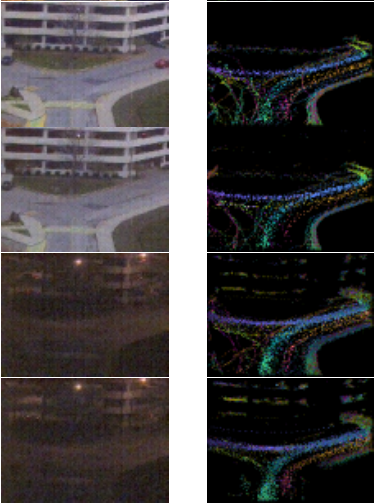
\includegraphics[scale=0.45]{tracker_4figs.png}
  \end{subfigure}\quad \begin{subfigure}[t!]{0.45\textwidth}
    \centering
    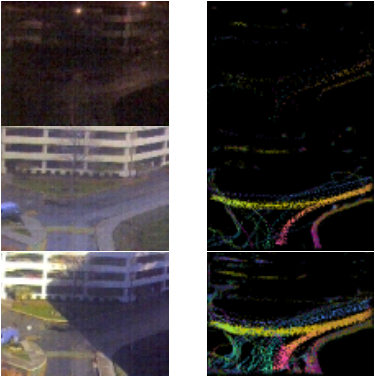
\includegraphics[scale=0.45]{tracker_3figs.png}
    \vspace{1.525cm}
  \end{subfigure}
      \vspace{-1mm}
  \caption*{Found trajectories in street scenario, colors indicate direction.}
\end{figure}
\end{frame}

\begin{frame}{Conclusion}

Authors conclude:
\begin{itemize}
\item Robust method for background subtraction
\item Handles lighting, slow changes, recurring motions
\item Real-time(!)
\item Difficulties arising from shortcomings in tracking methods
\end{itemize}

Future work
\begin{itemize}
\item Use full covariance matrix
\item Predict Gaussian changes (Kalman filter/PID controller)
\end{itemize}
\end{frame}

\begin{comment}
\begin{frame}[allowframebreaks]{References}
	\bibliographystyle{apalike}
	\bibliography{report}
\end{frame}
\end{comment}

\end{document}
